\documentclass[11pt,a4paper,english]{article}
  \usepackage[latin1]{inputenc}
  \usepackage{amsmath,amsfonts,amssymb}
  \usepackage{amsbsy}
  \usepackage{etoolbox}
  \usepackage{fullpage}
  \usepackage{graphicx}
  \usepackage{hyperref}
  \usepackage{minted}
  \usepackage{parskip}
  \usepackage[title]{appendix}
  \graphicspath{ {./} }

  \title{Bayesian Data Analysis - Assignment 1}
  \author{}

  \begin{document}
    \maketitle
    \definecolor{bg}{rgb}{0.95,0.95,0.95}

    \begin{enumerate}
      \item {\bf Basic probability theory notation and terms}
        \begin{itemize}
          \item[a)] Explanations:
            \begin{itemize}
              \item {\it probability}
                is the estimation of the possibility that an event will occur.
              \item {\it probability mass}
                refers to the probability of samples on an interval; eg. the entire probability
                sample space is equal to 1.
              \item {\it probability density}
                is the probability of mass divided by unit of the sample space.
              \item {\it probability mass function (pmf)}
                gives the probabilities of the possible values for a discrete random variable.
              \item {\it probability density function (pdf)}
                is a function of a continuous random variable, whose integral across an interval gives
                the probability that the value of the variable lies within the same interval.
              \item {\it probability distribution}
                is a function of a discrete variable whose integral over any interval is the probability
                that the variate specified by it will lie within that interval.
              \item {\it discrete probability distribution}
                refers to the probability of occurrence of each value of a discrete random variable.
              \item {\it continuous probability distribution}
                refers to the probabilities of the possible values of a continuous random variable.
              \item {\it cumulative distribution function (cdf)}
                calculates the cumulative probability for a given x-value and it can be used to determine
                the probability that a random observation that is taken from the sample space will be less
                than or equal to a certain value.
              \item {\it likelihood}
                is a function of the parameters of a statistical model, given specific observed data.
            \end{itemize}

          \item[b)] Answers to the questions:
            \begin{itemize}
              \item {\it What is observation model?}\\
                Observation model refers to the expression that relates the parameters of the
                model to the observations.
              \item {\it What is statistical model?}\\
                Statistical modeling is a mathematically simplified way to approximate reality
                and optionally to make predictions from this approximation.
              \item {\it What is the difference between mass and density?}\\
                Mass refers to the entire sample space, whereas density is the fraction from that
                sample space.
            \end{itemize}
        \end{itemize}

      \item {\bf Basic computer skills}
        \begin{itemize}
          \item[a)] Plot the density function
            \begin{minted}[bgcolor=bg,linenos,fontsize=\small,autogobble]{python}
              from scipy import stats
              import numpy
              import matplotlib
              import matplotlib.pyplot as plt

              MEAN = 0.2
              VARIANCE = 0.01

              fig, axis = plt.subplots(1, 1)

              alfa = MEAN * ( (MEAN * (1 - MEAN) / VARIANCE) - 1 )
              beta = alfa * (1 - MEAN) / MEAN

              x_range = numpy.linspace(0, 1, 100)
              y_range = stats.beta.pdf(x_range, alfa, beta)

              axis.plot(x_range, y_range)
            \end{minted}
            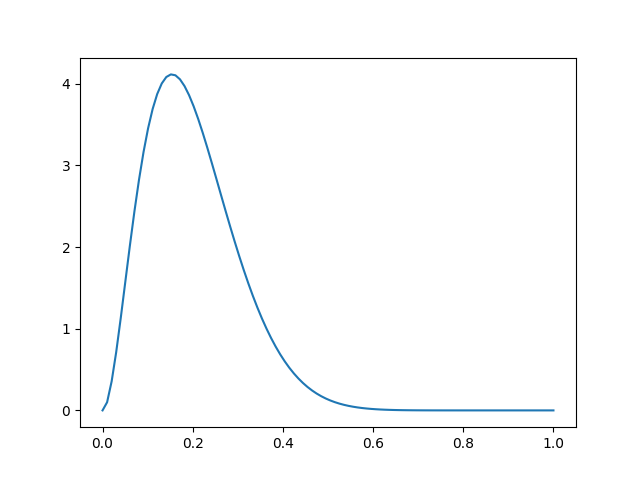
\includegraphics[width=10cm]{prob_distribution.png}

          \item[b)] Take a sample of 1000 random numbers and plot a histogram of the results
            \begin{minted}[bgcolor=bg,linenos,fontsize=\small,autogobble]{python}
              random_samples = stats.beta.rvs(alfa, beta, size=1000)
              axis.hist(random_samples, density=True, alpha=0.5)
            \end{minted}
            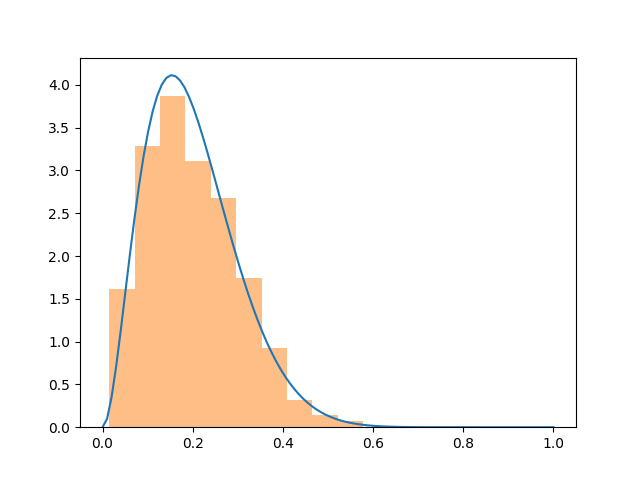
\includegraphics[width=10cm]{prob_distribution_hist.png}

          \item[c)] Compute the sample mean and variance from the drawn sample
            \begin{minted}[bgcolor=bg,linenos,fontsize=\small,autogobble]{python}
              sample_mean = numpy.mean(random_samples)
              sample_variance = numpy.var(random_samples)
              print('sample mean: ', sample_mean)
              print('sample variance: ', sample_variance)
            \end{minted}

            \begin{minted}[bgcolor=bg,fontsize=\small,autogobble]{text}
              $ sample mean:  0.19997418955672838
              $ sample variance:  0.01045597802573812
            \end{minted}

          \item[d)] Estimate the central 95\%-interval of the distribution
            \begin{minted}[bgcolor=bg,linenos,fontsize=\small,autogobble]{python}
              sample_percentile = numpy.percentile(random_samples, q=97.5)
              print('sample central percentile 95%: ', sample_percentile)
            \end{minted}

            \begin{minted}[bgcolor=bg,fontsize=\small,autogobble]{text}
              $ sample central percentile 95%:  0.4188436088624379
            \end{minted}
        \end{itemize}

      \item {\bf Bayes' theorem}:
        How would you advice a group of researchers who designed a new test for detecting lung cancer?

        \begin{math}
          P(Person_{randomly\ selected\ and\ has\ cancer} | Positive\ result) = \\
          = \frac{P(P_{has\ cancer}) * P(Cancer)}{P(Positive\ result)} = \frac{0.98 * 0.001}{0.98 * 0.001 + 0.04*0.999}
          = 0.023
        \end{math}

        The result of test is not very satisfying for a randomly selected person who has cancer. Thus, I would tell the
        researchers to make their test prediction better.

      \item {\bf Bayes' theorem}:
        Find the probability of the selected ball being red and the box it came from.\\
        \begin{math}
          A = 2_{red}\ 5_{white};\ selected\ 40\%\ of\ the\ time \\
          B = 4_{red}\ 1_{white};\ selected\ 10\%\ of\ the\ time \\
          C = 1_{red}\ 3_{white};\ selected\ 50\%\ of\ the\ time \\
          \\
          P(red) = 0.4 * \frac{2}{7} + 0.1 * \frac{4}{5} + 0.5 * \frac{1}{4} = 0.319\\
          \\
          P(A|red) = \frac{P(red\ from\ A) * P(A)}{P(red)} = \frac{\frac{2}{7} * 0.4}{0.319} = 0.358\\
          \\
          P(B|red) = \frac{P(red\ from\ B) * P(B)}{P(red)} = \frac{\frac{4}{5} * 0.1}{0.319} = 0.250\\
          \\
          P(C|red) = \frac{P(red\ from\ C) * P(C)}{P(red)} = \frac{\frac{1}{4} * 0.5}{0.319} = 0.391\\
        \end{math}
        The probability of a red ball being picked is 31.9\% and there is 39.1\% chance that it came from Box C.

      \item {\bf Bayes' theorem}:
        What is the probability that Elvis was an identical twin?\\
        Let's assume that: \begin{math}S_{gt}\end{math} is a notation of same gender twins,
        \begin{math}I_t\end{math} stands for identical twins and \begin{math}F_t\end{math} means
        fraternal twins. We need to find \begin{math}P(I_t|S_{gt})\end{math}.

        \begin{math}
          P(S_{gt}) = P(I_t) + P(F_t\ for\ the\ same\ gender) = \frac{1}{300} + 0.5 * \frac{1}{125} = 0.0073\\
          P(I_t|S_{gt}) = \frac{P(Elvis\ being\ twin) * P(I_t)}{S_{gt}} = \frac{1 * \frac{1}{300}}{0.0073} = 0.45
        \end{math}
        \\
        There is 45\% chance that Elvis was an identical twin.
    \end{enumerate}

    \begin{appendices}
      \section{Source code}
      \begin{minted}[bgcolor=bg,linenos,fontsize=\small,autogobble]{python}
        from scipy import stats
        import numpy
        import matplotlib
        matplotlib.use('TkAgg')
        import matplotlib.pyplot as plt

        MEAN = 0.2
        VARIANCE = 0.01
        fig, axis = plt.subplots(1, 1)

        alfa = MEAN * ( (MEAN * (1 - MEAN) / VARIANCE) - 1 )
        beta = alfa * (1 - MEAN) / MEAN

        x_range = numpy.linspace(0, 1, 100)
        y_range = stats.beta.pdf(x_range, alfa, beta)

        # a) Plot the density function of Beta-distribution
        axis.plot(x_range, y_range)
        fig.savefig('./ex1/prob_distribution.png')

        # b) Take a sample of 1000 random numbers and plot a histogram
        random_samples = stats.beta.rvs(alfa, beta, size=1000)
        axis.hist(random_samples, density=True, alpha=0.5)
        fig.savefig('./ex1/prob_distribution_hist.png')

        # c) Compute the sample mean and variance from the drawn sample
        sample_mean = numpy.mean(random_samples)
        sample_variance = numpy.var(random_samples)
        print('sample mean: ', sample_mean)
        print('sample variance: ', sample_variance)

        # d) Estimate the central 95%-interval from the drawn samples
        sample_percentile = numpy.percentile(random_samples, q=97.5)
        print('sample central percentile 95%: ', sample_percentile)
      \end{minted}
    \end{appendices}
  \end{document}
